\section{命令行模式下的 Nsight Compute 性能分析}

\section*{前言}
欢迎大家。在今天的文章中，我将解释如何使用 \textbf{Nsight Compute} 工具来分析任何 CUDA应用
程序，该工具由 NVIDIA 提供。不过在文章开始前，我想先说明一点：任何公司的性能分析工具都应提供两种分析方法。

\begin{enumerate}
    \item \textbf{命令行分析 (CLI Profiling)}：正如我们这里看到的，我们可以使用一些命令来收集特定指标以评估 CUDA 应用程序的性能。
    \item \textbf{图形用户界面分析 (GUI Profiling)}：今天我将从第一种方法即命令行分析开始。在另一个文章中，我将详细讲解 GUI 分析。
\end{enumerate}

这两种方法都非常重要。有时你可能只需要收集几个指标来评估特定硬件单元的性能，在这种情况下，最佳选择可能就是命令行分析。但
如果你想进行深入的性能评估，最好使用GUI 分析，因为它可以为你提供诸如性能屋顶线分析 (RooflineAnalysis)、图表以及每个硬件单元的利用率等信息。


\subsection{文档与基础命令}
像我们通常做的那样，我将打开文档先大致了解一下命令行分析。你需要做的就是搜索 ``Nsight ComputeCLI''
并打开第一个链接。该网页包含了关于 Nsight Compute 命令行分析你需要知道的一切。

基础命令如下：
\begin{lstlisting}
ncu --set full -o profile ./my_cuda_app
\end{lstlisting}
如果你正在使用 MPI，你可以针对特定进程或者针对所有进程进行分析。此外，你还可以指定输出文件、分段文件夹，或过滤想要分
析的核函数(Kernel)。


\begin{figure}
    \centering
    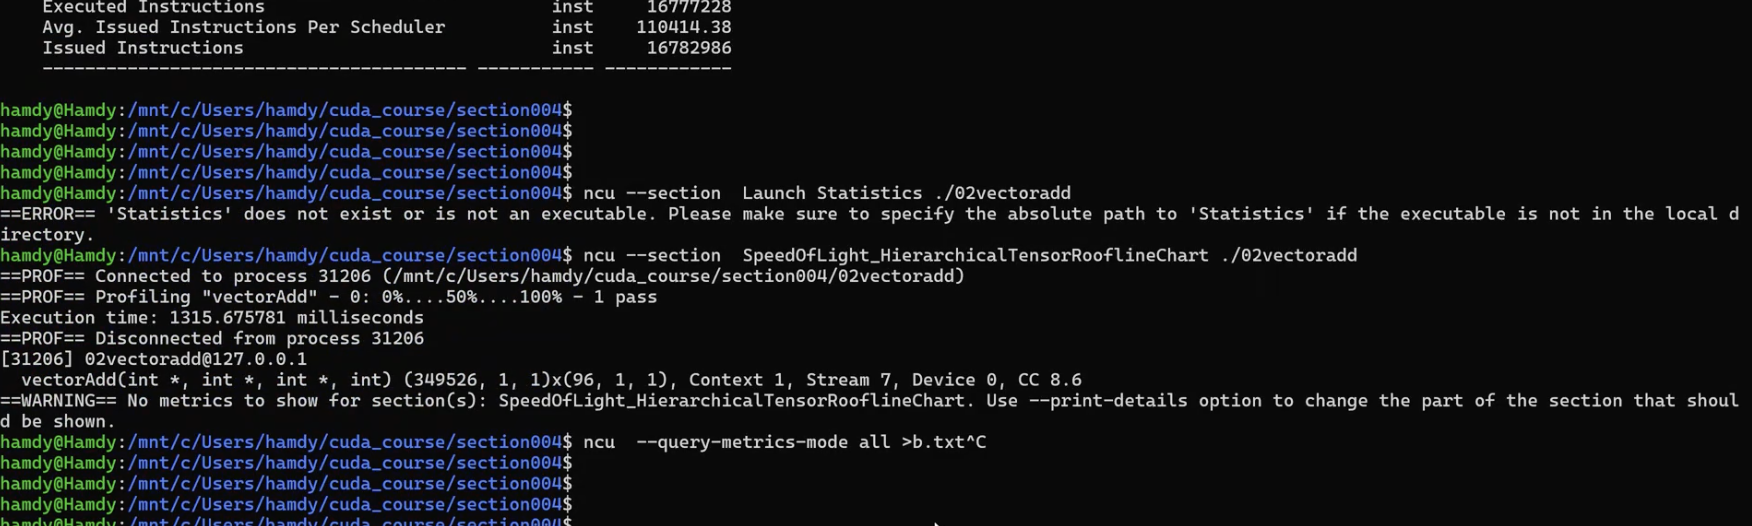
\includegraphics[width=0.75\linewidth]{resources/cuda-102.png}
    \caption{}
    \label{fig:placeholder}
\end{figure}

\subsection{分段 (Sections)}
Nsight Compute 将分析数据组织为不同的``分段''。当我们运行最简单的 \texttt{ncu}命令时，默
认会显示四个分段：
\begin{enumerate}
    \item \textbf{GPU Performance Ceiling (GPU 性能上限)}：显示 GPU 中不同单元的吞吐量信息。
    \item \textbf{Launch Statistics (启动统计)}：包含 DRAM 吞吐量、L1 和 L2 缓存吞吐量、流式多处理器 (SM) 利用率等。
    \item \textbf{Occupancy (占用率)}：包含块大小、网格大小、每个线程的寄存器数量、每个 SM 使用的共享内存大小等。
    \item \textbf{GPU and Memory Workload Distribution (GPU 与内存工作负载分布)}：显示理论占用率与实际占用率（例如本例中实际占用率为 81\%），以及 DRAM、L1、L2 缓存等的活跃周期数。
\end{enumerate}

Nsight Compute 实际上包含约 23 个分段（从 ID 4 到 27）。在命令行中，我们需要使用分段的标识符
(ID) 而非显示名称。例如，若只想查看``Launch Statistics''，可使用：
\begin{lstlisting}
ncu --section LaunchStats ./my_cuda_app
\end{lstlisting}
其他分段还包括 NVLink 通信统计、调度器统计 (Scheduler Stats)、线程束状态统计 (WarpState Stats) 等。


\subsection*{分析建议与警告}
Nsight Compute 有时会提供建议或警告。例如提示``可选指标无法找到''，这可能是因为当前 GPU架构不支持
该指标。另外，工具可能会给出停顿原因分析，例如：``平均而言，此核函数的每个线程束因等待记分牌依赖(ScoreboardDependency) 而停顿了 111个周期''。理解这些信息需要结合总周期数来判断瓶颈严重程度。


\subsection{指标 (Metrics)}
Nsight Compute 包含海量指标（约 10 万个）。为了高效使用，需掌握其命名规则。

\subsection{指标命名结构}
指标名称通常遵循以下格式：
\begin{center}
    \texttt{<硬件单元>\_\_<指标描述>.<聚合方式>}
\end{center}

\begin{figure}
    \centering
    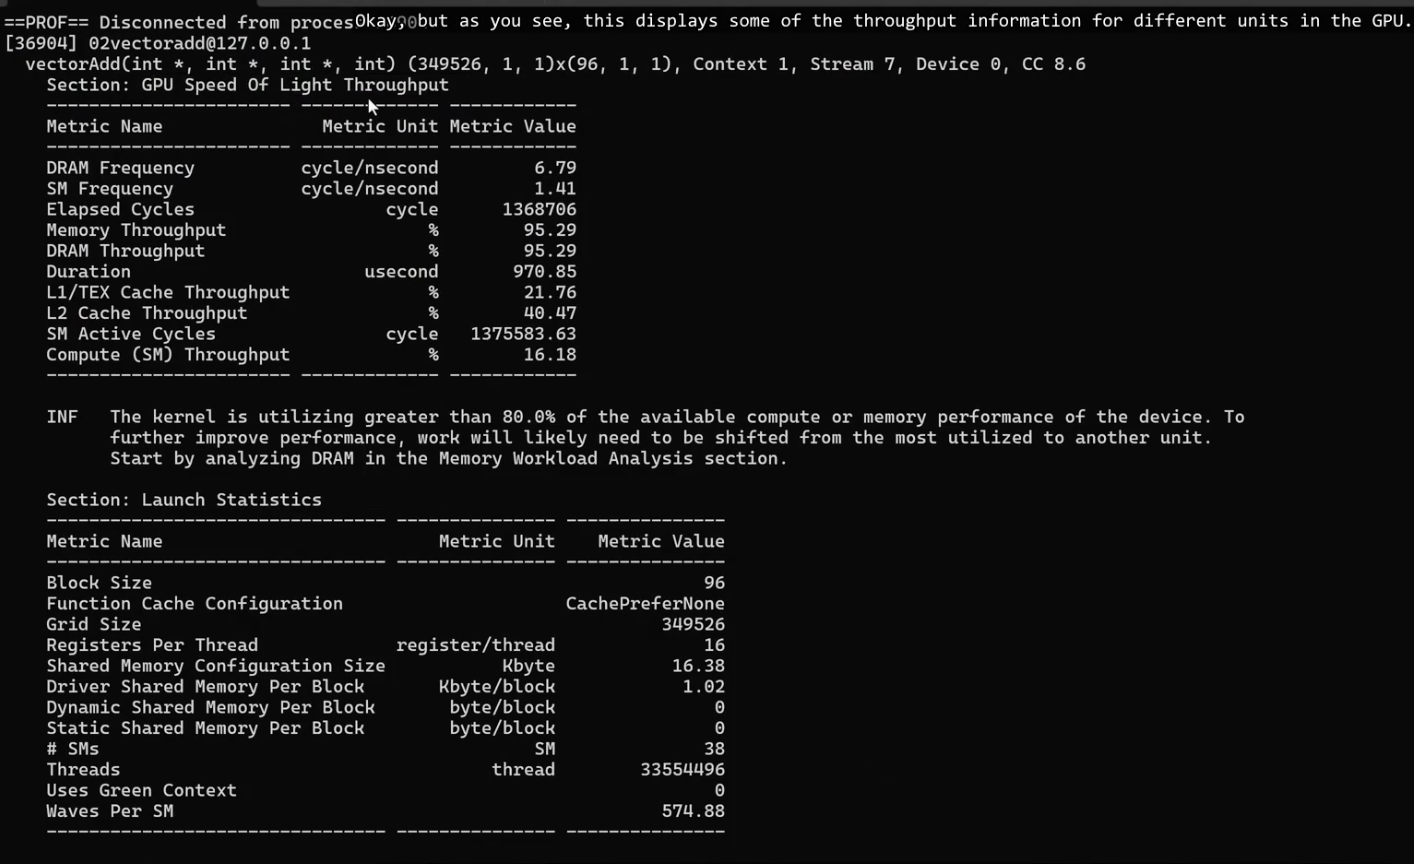
\includegraphics[width=0.75\linewidth]{resources/cuda-103.png}
    \caption{}
    \label{fig:placeholder}
\end{figure}

\subsection{硬件单元前缀}
双下划线之前的部分定义了被分析的硬件单元：
\begin{itemize}
    \item \texttt{dram}: 设备内存 (DRAM)
    \item \texttt{l1tex}: L1/纹理缓存
    \item \texttt{lts}: L2 缓存 (Level Two Slice)
    \item \texttt{sm}: 流式多处理器 (Streaming Multiprocessor)
    \item \texttt{gpu}: 整个 GPU
\end{itemize}

\subsection{聚合方式后缀}
点号 (\texttt{.}) 之后的标识符表示数据的聚合方式：
\begin{itemize}
    \item \texttt{.min}: 所有 SM 中的最小值
    \item \texttt{.max}: 所有 SM 中的最大值
    \item \texttt{.avg}: 所有 SM 的平均值
    \item \texttt{.sum}: 整个 GPU 的总和
\end{itemize}

\noindent \textbf{重要技巧：} \texttt{.sum} 是基于最大值计算的，而非平均值。即：$\text{Sum} = \text{Max} \times \text{SM\_Count}$。如果在命令行中省略点号及后缀（例如只写 \texttt{smsp\_inst\_executed}），工具将自动收集该指标的所有聚合类型（avg, max, min, sum）。
\subsection{常用指标示例}
\begin{itemize}
    \item \textbf{L1 缓存命中率}: \texttt{l1tex\_hit\_rate}
    \item \textbf{DRAM 访问字节数}: \texttt{dram\_bytes.sum}
    \item \textbf{扇区数量}: NVIDIA GPU 中每个扇区 (Sector) 为 32 字节。相关指标如 \texttt{dram\_sectors.read.sum}。
    \item \textbf{指令执行数}: \texttt{smsp\_inst\_executed.avg} (SM 内执行的平均指令数)。
    \item \textbf{管道利用率}: 可搜索 \texttt{pipe\_lsu} (加载存储单元)、\texttt{pipe\_tensor} (张量核心)、\texttt{fp16} / \texttt{fp64} 等。
\end{itemize}

\subsection{实战应用与导出}
\subsection{收集特定指标}
我们可以使用 \texttt{--metrics} 参数收集指定指标：
\begin{lstlisting}
ncu --metrics l1tex__hit_rate,smsp__inst_executed ./02_vector_add
\end{lstlisting}
如果 L1 命中率为 0\%，说明所有内存操作都访问了全局内存，这是严重的性能瓶颈，需要优化数据局部性。

\begin{figure}
    \centering
    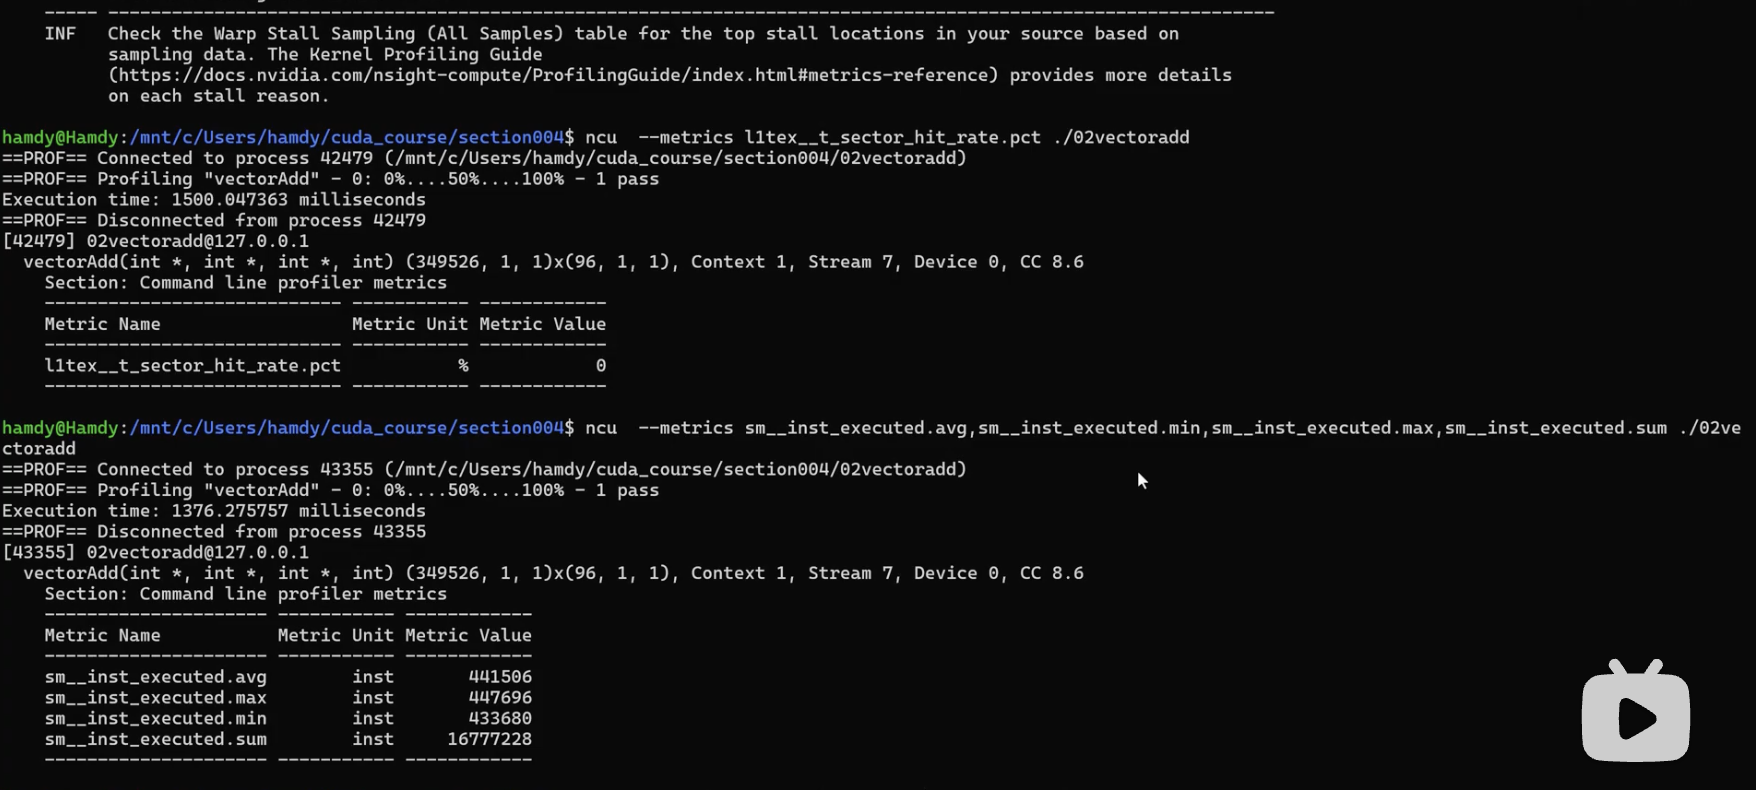
\includegraphics[width=0.75\linewidth]{resources/cuda-104.png}
    \caption{}
    \label{fig:placeholder}
\end{figure}

\subsection{使用正则表达式过滤}
若要分析特定硬件单元的所有指标，可使用正则表达式：
\begin{lstlisting}
ncu --metrics ".*shared.*" ./02_vector_add
\end{lstlisting}
这将筛选出所有包含 ``shared'' 的指标（如共享内存相关指标）。

\subsection{导出结果}
可以将分析结果导出为 CSV 文件以便在 Excel 中查看：
\begin{lstlisting}
ncu --metrics smsp__inst_executed --csv --log-file result.csv ./app
\end{lstlisting}
导出的表格包含指标名称、单位、以及各聚合方式对应的数值。

\section*{结语}
今天我们学习了如何使用 Nsight Compute命令行工具进行基础性能评估，包括分段的选择、指标的命名规则解析以及结
果导出。在后续文章中，我们将应用这些知识，通过特定指标深入分析代码，例如探究块数和线程数对核函数执行时间及周期数的具体影
响。

